\graphicspath{{chapter1/}{manuscript/}}

\chapter{\textbf{}}

\begin{center}
\textbf{Paying colonization credit with forest management could
accelerate the range shift of temperate trees under climate change} \\
Willian~Vieira, Isabelle~Boulangeat, Marie-Hélène~Brice, Robert
L.~Bradley, Dominique~Gravel
\end{center}

\hypertarget{supplementary-material-1}{%
\section{Supplementary Material 1}\label{supplementary-material-1}}

\hypertarget{fig:sim-result-supp1_ch1}{%
\begin{figure}
\centering
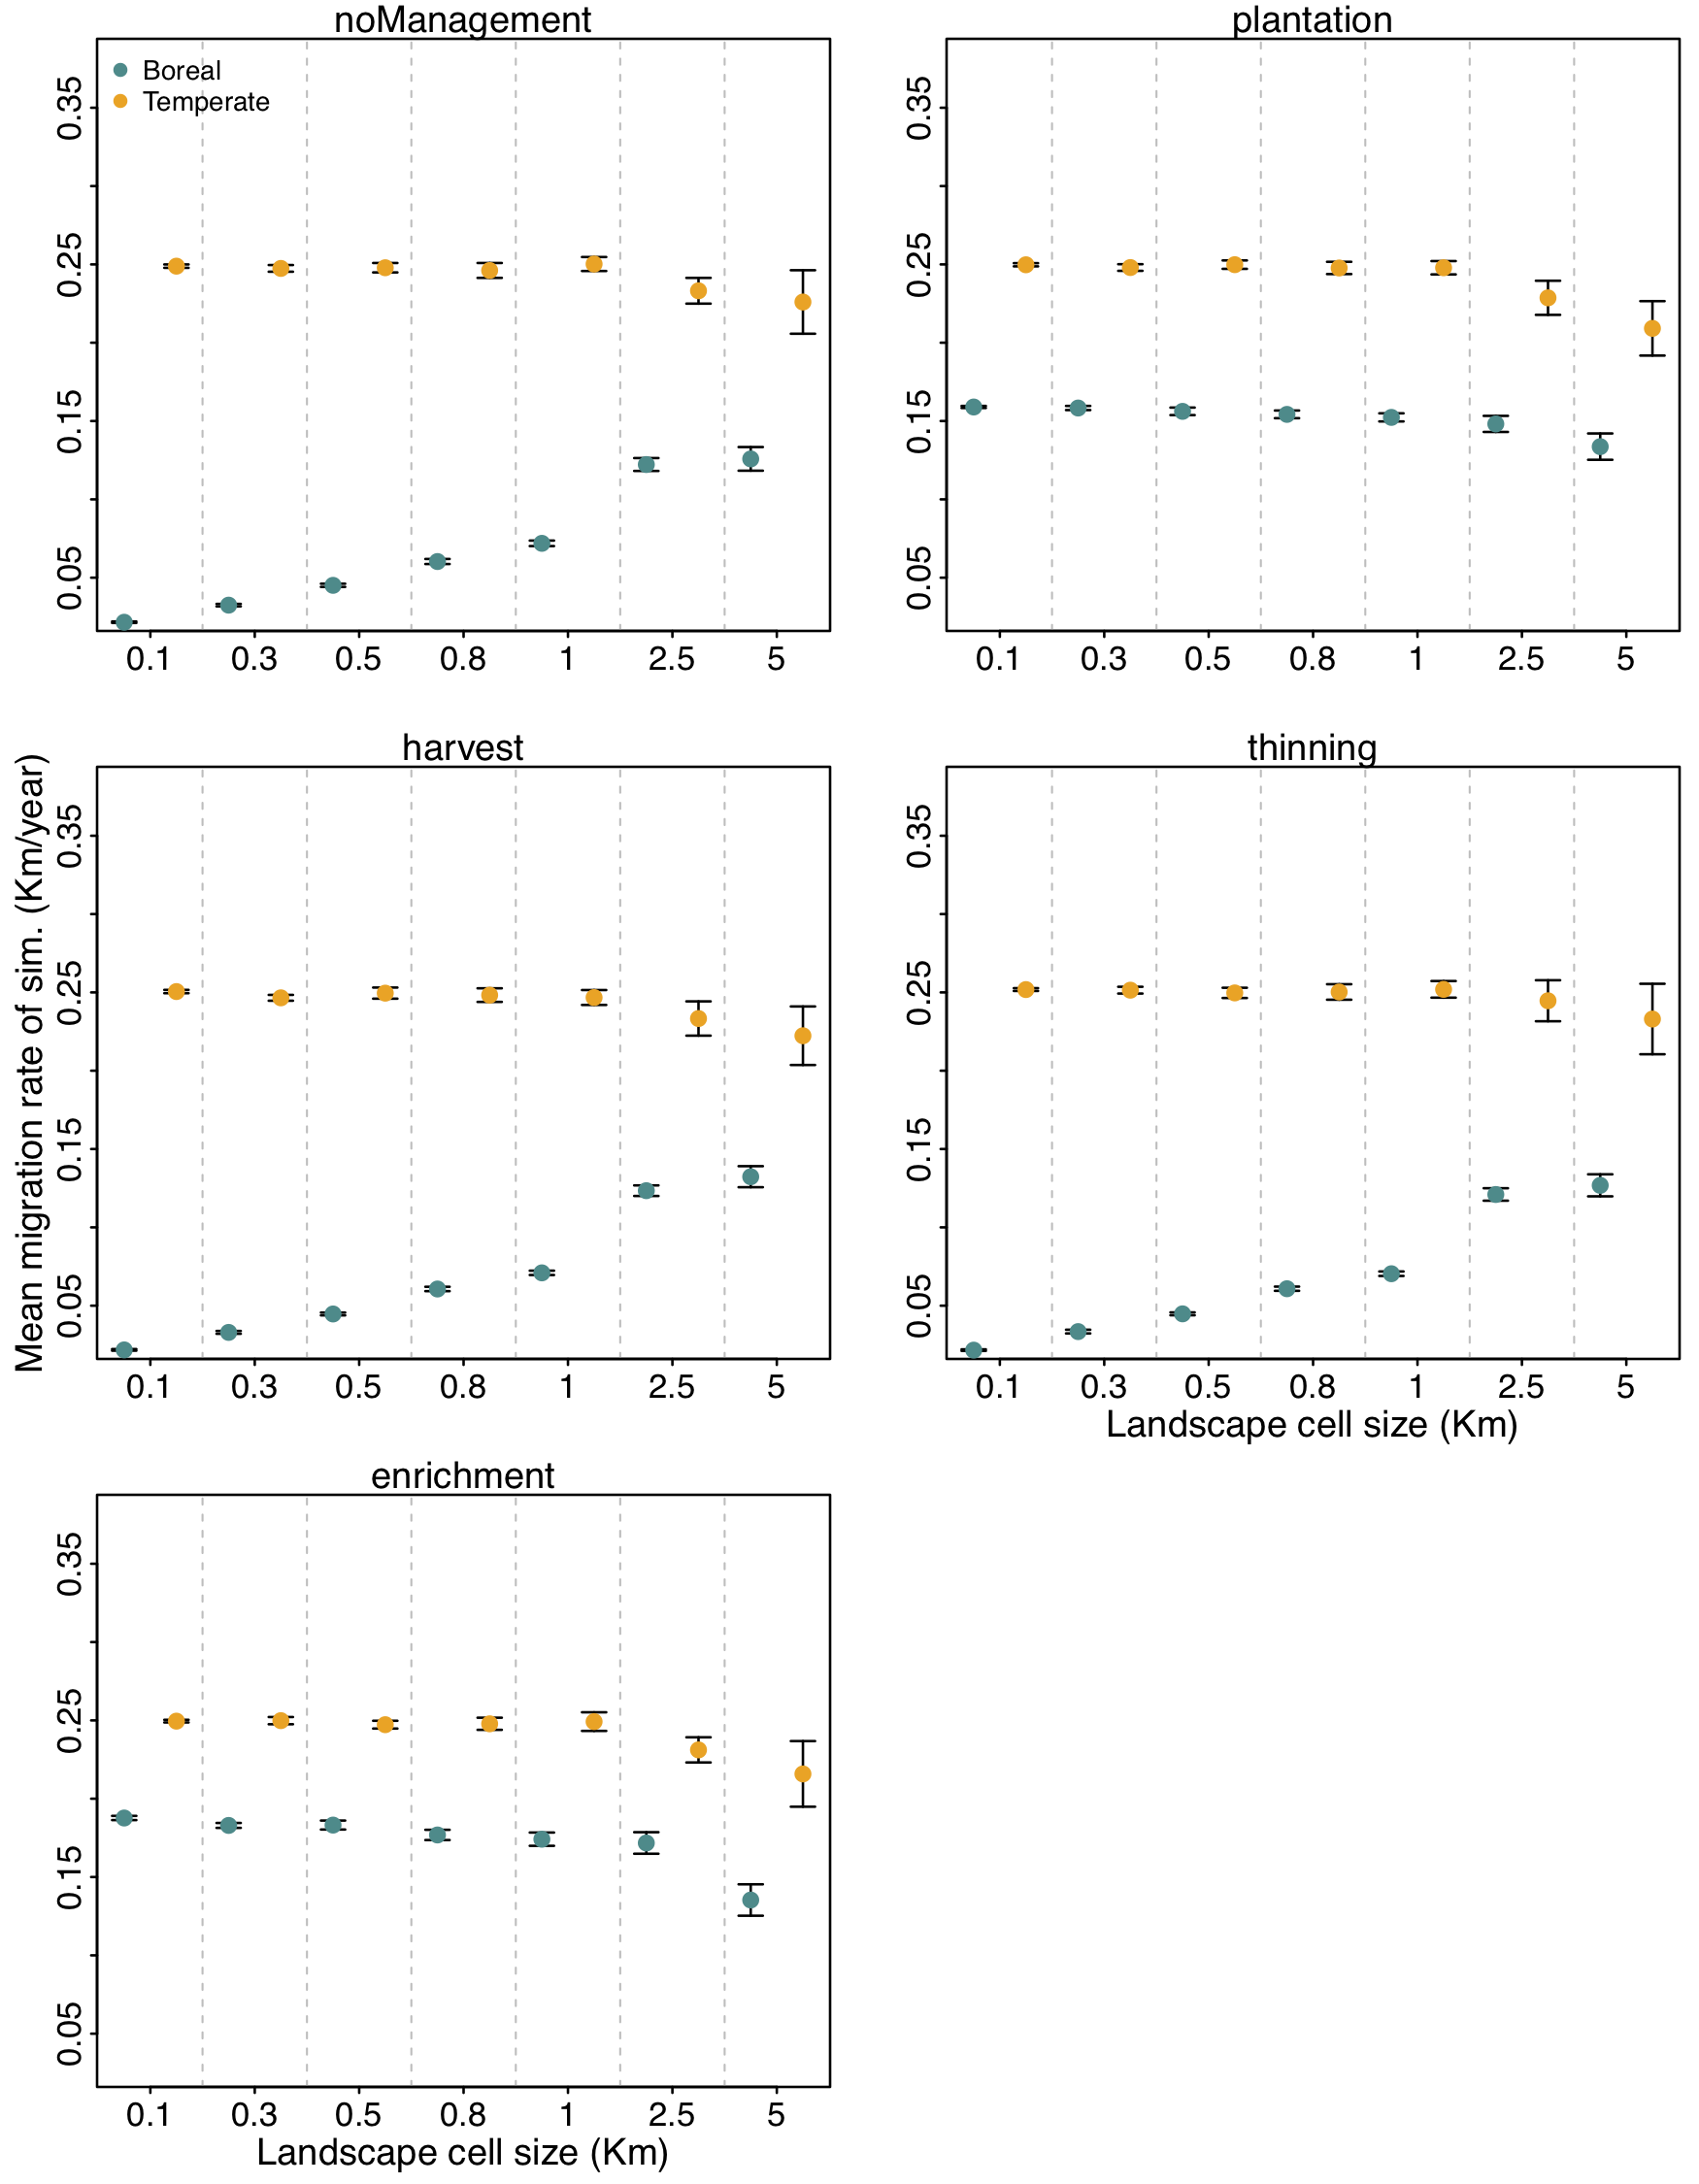
\includegraphics[width=0.65\textwidth,height=\textheight]{manuscript/figs/58586171-78e3ab80-8228-11e9-9fa5-ec8354eae439.png}
\caption[{Sensitivity analysis of the effect of cell size on dispersal
rate for different management practices.}]{Sensitivity analysis of the
effect of cell size on dispersal rate for different management
practices. For each cell size ranging from 0.1 Km (1 ha) to 5 km (2500
ha), we warmed temperature with RCP4.5 increasing linearly for the first
100 years, and let the model run for a total of 1000 years. We specified
the range limit of a forest state within the landscape grid when the
occupancy of the state was less than 85\%. The mean migration rate of a
simulation is therefore defined as the distance the range limit of a
forest state travelled, divided by the total amount of time. Note that
the values of migration rate are may not be realistic, as they are
dependent on the size of the theoretical landscape lattice, but are
enough to compare between the different cell sizes. More information
about this analysis can be found here:
\url{https://github.com/willvieira/STManaged/issues/1}}
\label{fig:sim-result-supp1_ch1}
\end{figure}
}

\newpage

\hypertarget{fig:sim-result-supp2_ch1}{%
\begin{figure}
\centering
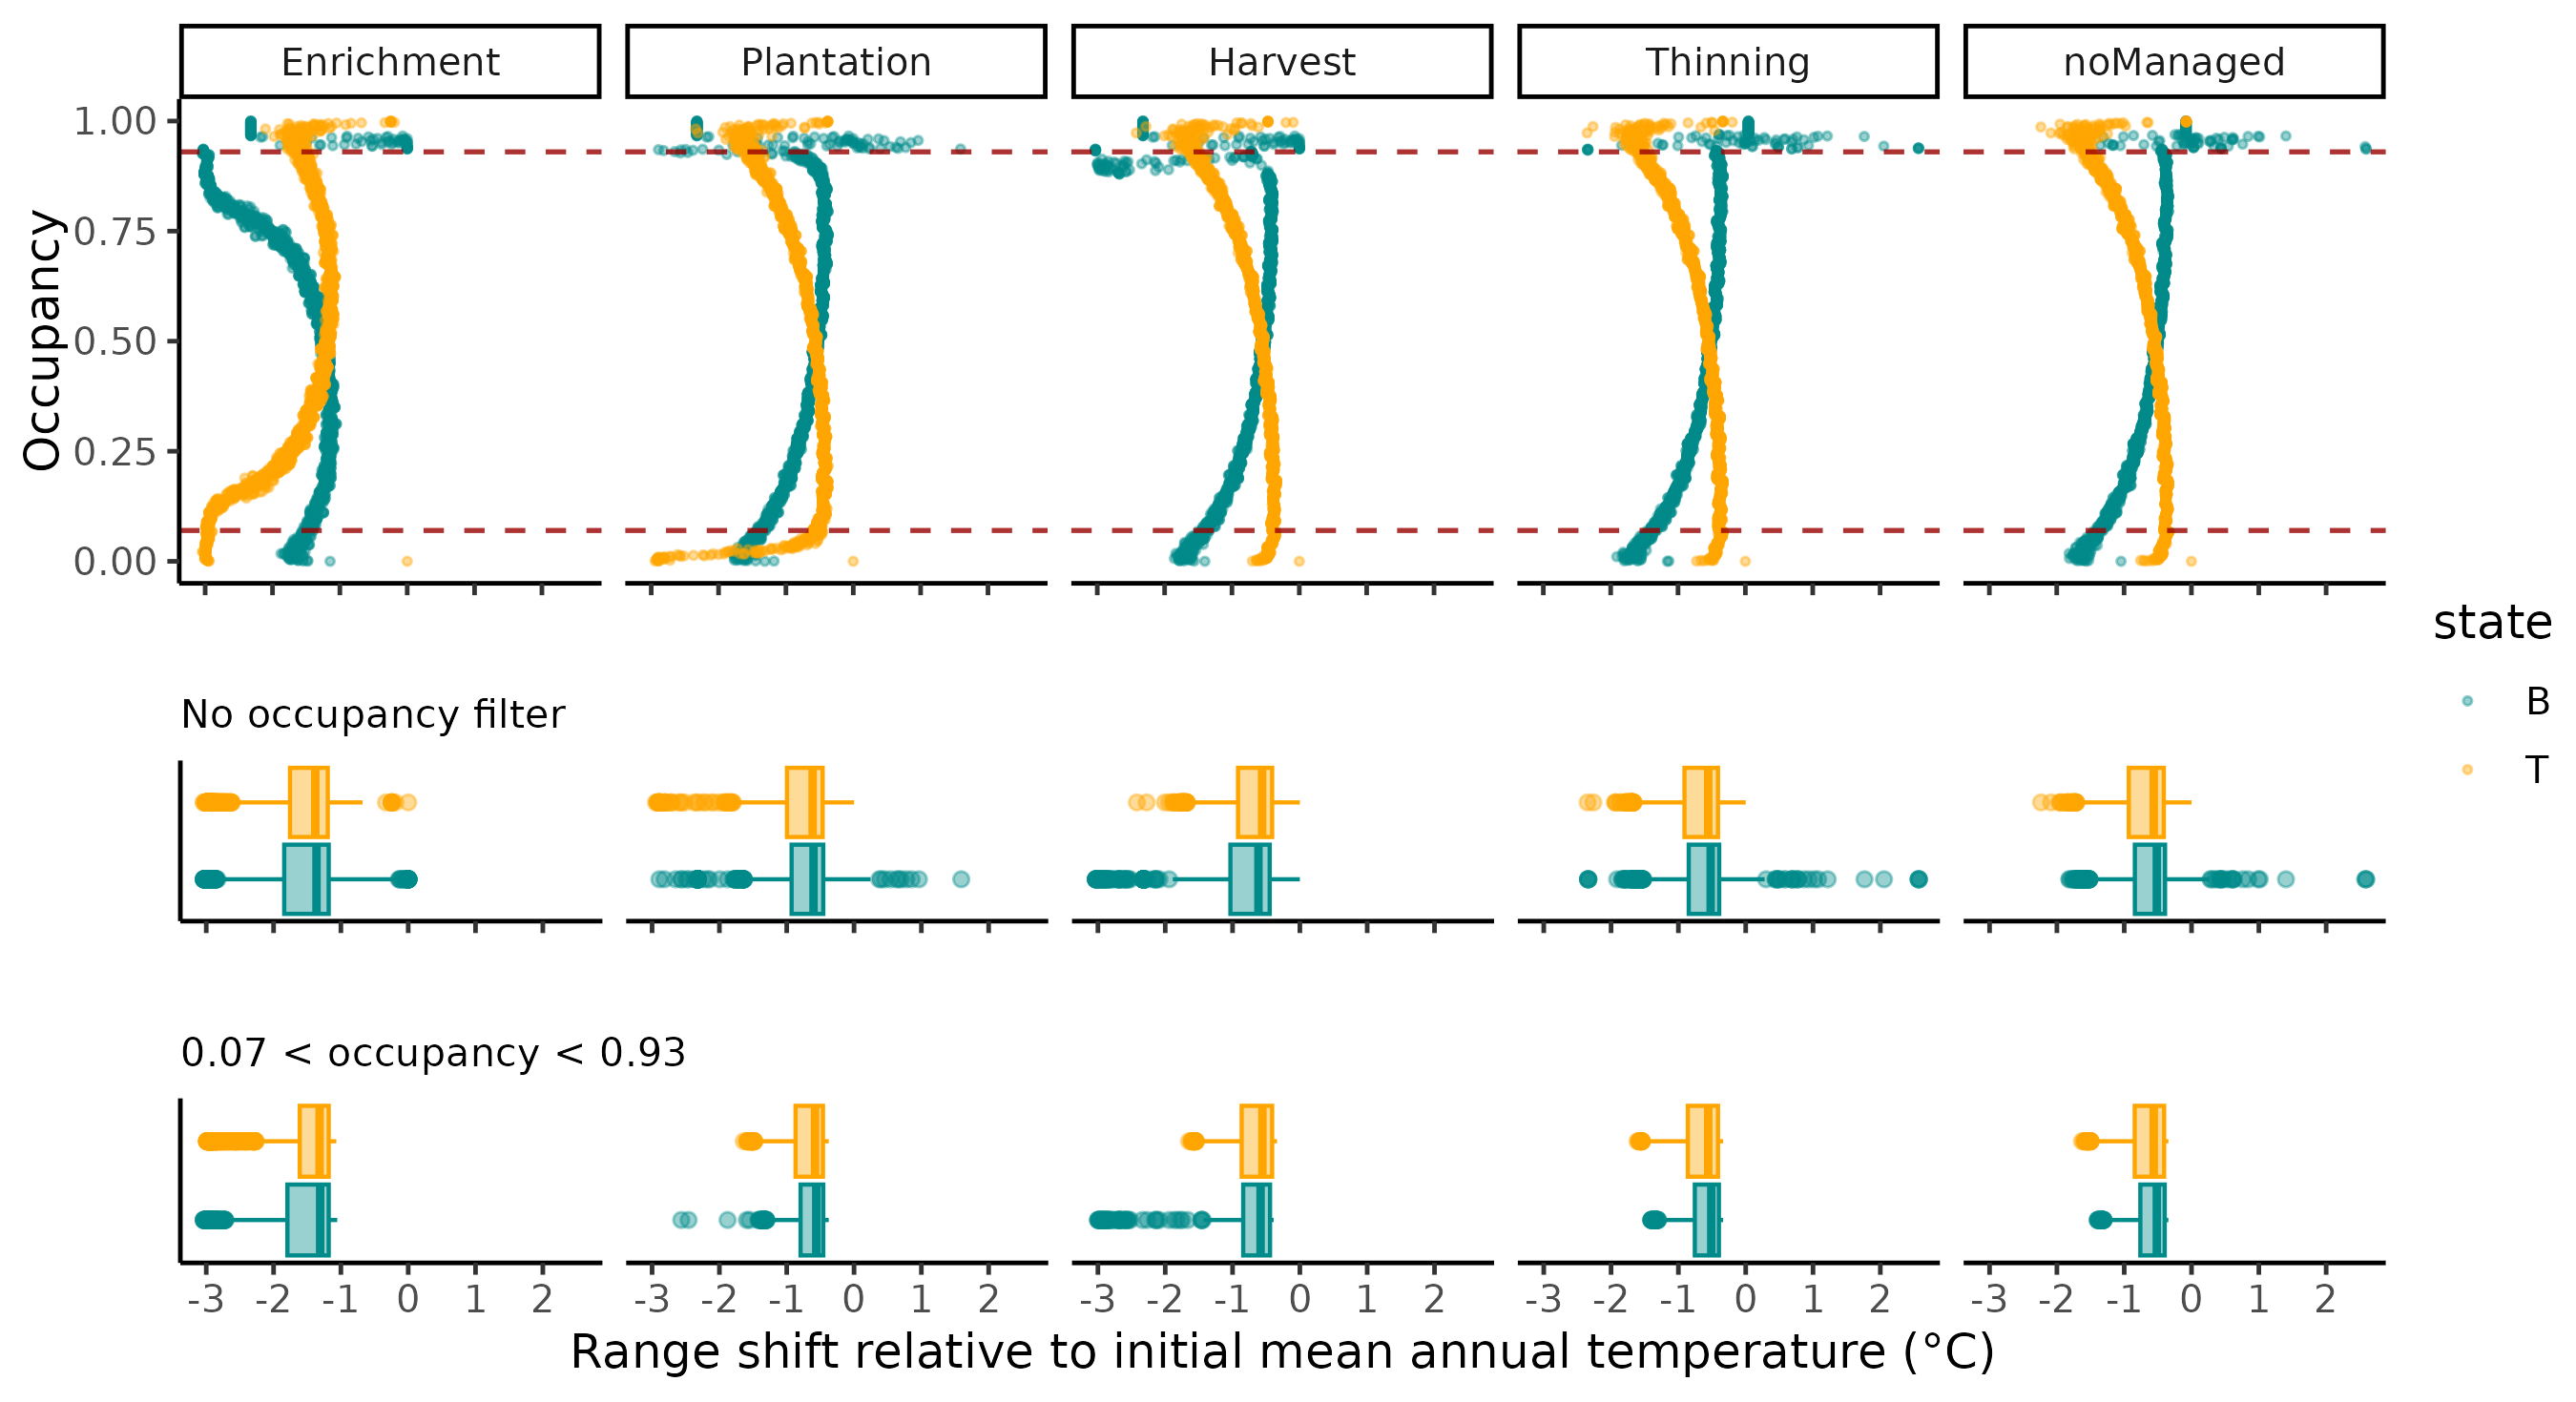
\includegraphics{manuscript/img/sim-result_supp5.png}
\caption[{Range shift relative to initial mean annual temperature for
the boreal (dark green) and temperate-mixed (orange) states.}]{Range
shift relative to initial mean annual temperature for the boreal (dark
green) and temperate-mixed (orange) states. Range shift was computed for
all values of occupancy {[}0-1{]} by calculating the difference between
initial state distribution (\(T_0\)), and the final distribution of a
simulation. The panels in the first row show the range shift in function
of occupancy for the median output of the \(T_{150}CC + FM\) simulation
(Figure 5). The panels in the second and third row test whether
filtering extreme occupancy values have an effect on the range shift
summary.}
\label{fig:sim-result-supp2_ch1}
\end{figure}
}

\newpage

\hypertarget{fig:sim-result-supp3_ch1}{%
\begin{figure}
\centering
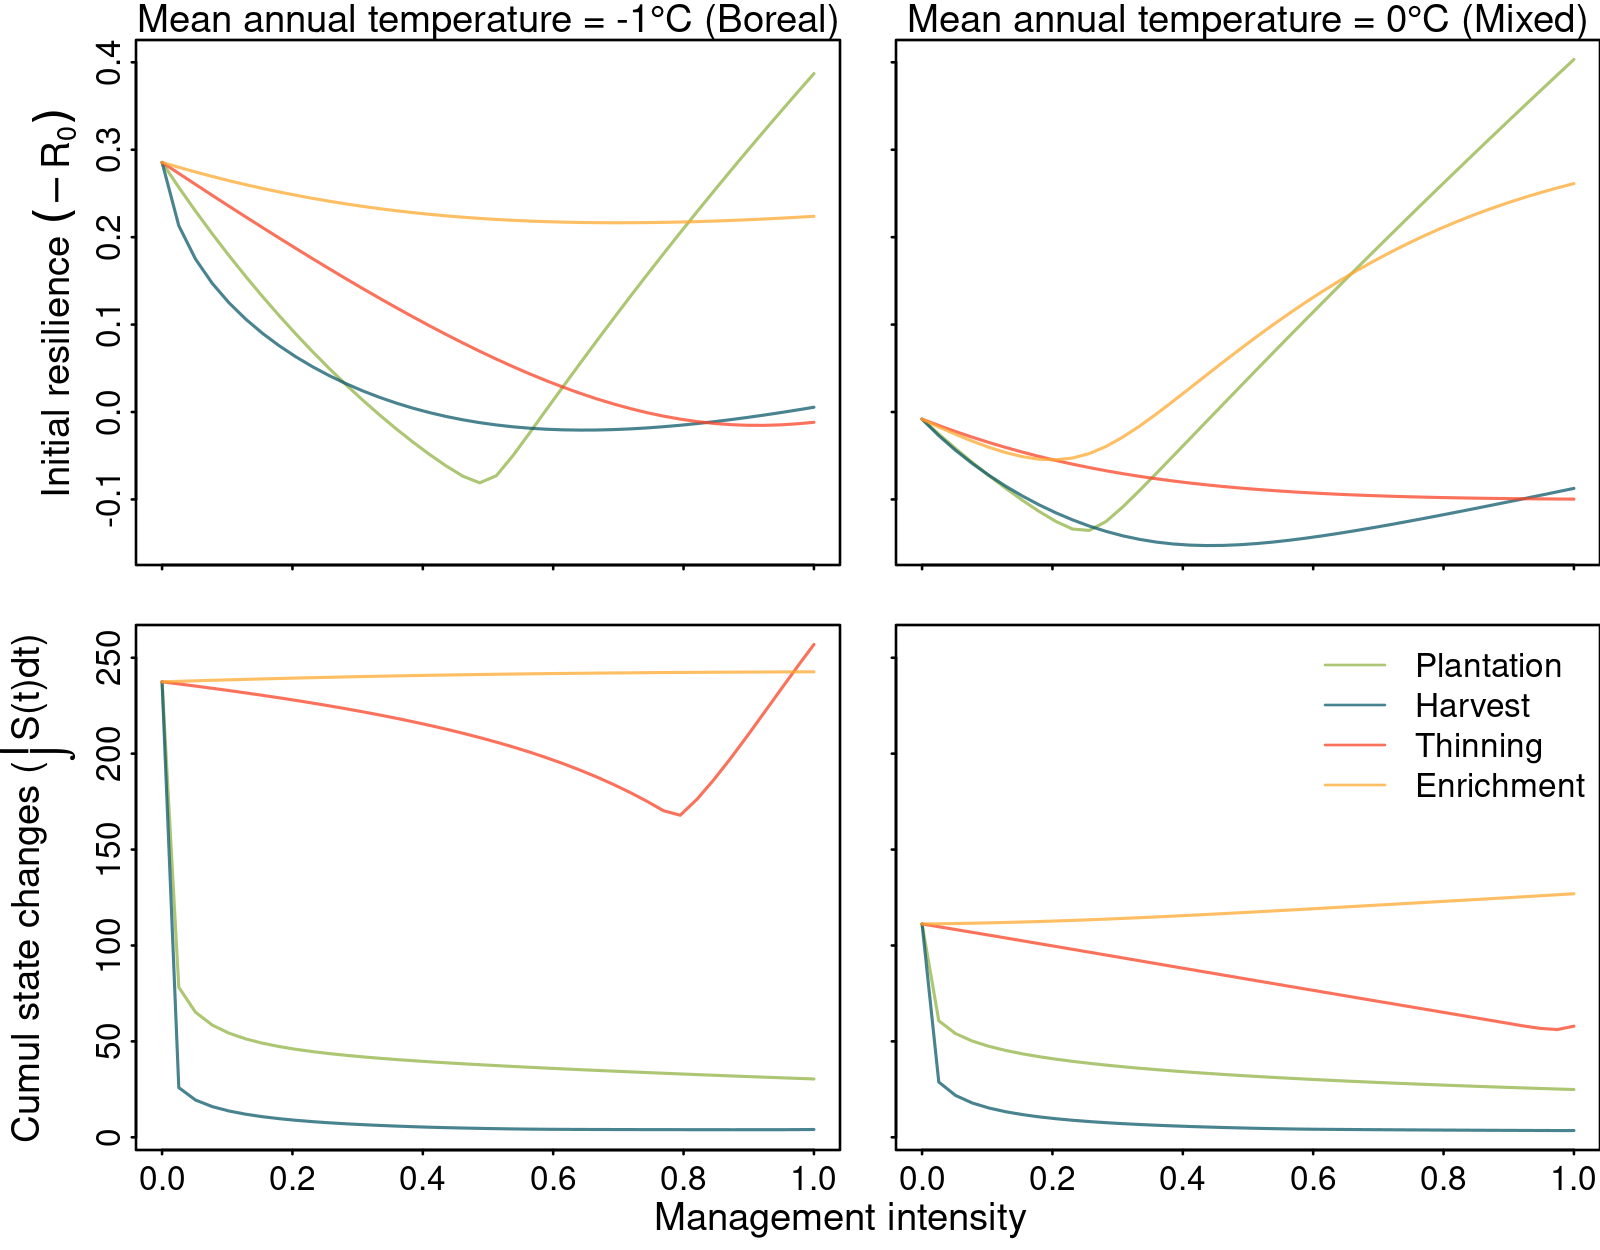
\includegraphics{manuscript/img/num-result_supp1.png}
\caption[{Transient dynamics following warming temperature along with
the increasing management intensity for plantation, harvest, thinning
and enrichment planting.}]{Transient dynamics following warming
temperature along with the increasing management intensity for
plantation, harvest, thinning and enrichment planting. Climatic
condition is fixed at the boreal (mean annual temperature of -1; left
panels) and the boreal/mixed transition (mean annual temperature of 0;
right panels) regions. Transient dynamics are described by (i) exposure
or the shift of forest states to the new equilibrium; (ii) asymptotic
resilience or the rate in which the system recovery to equilibrium;
(iii) sensitivity or the time for the state reach equilibrium after
warming temperature; (iv) initial resilience or the reactivity of the
system after warming temperature; and (v) vulnerability or the
cumulative amount of state changes after warming temperature.}
\label{fig:sim-result-supp3_ch1}
\end{figure}
}

\newpage

\hypertarget{fig:sim-result-supp4_ch1}{%
\begin{figure}
\centering
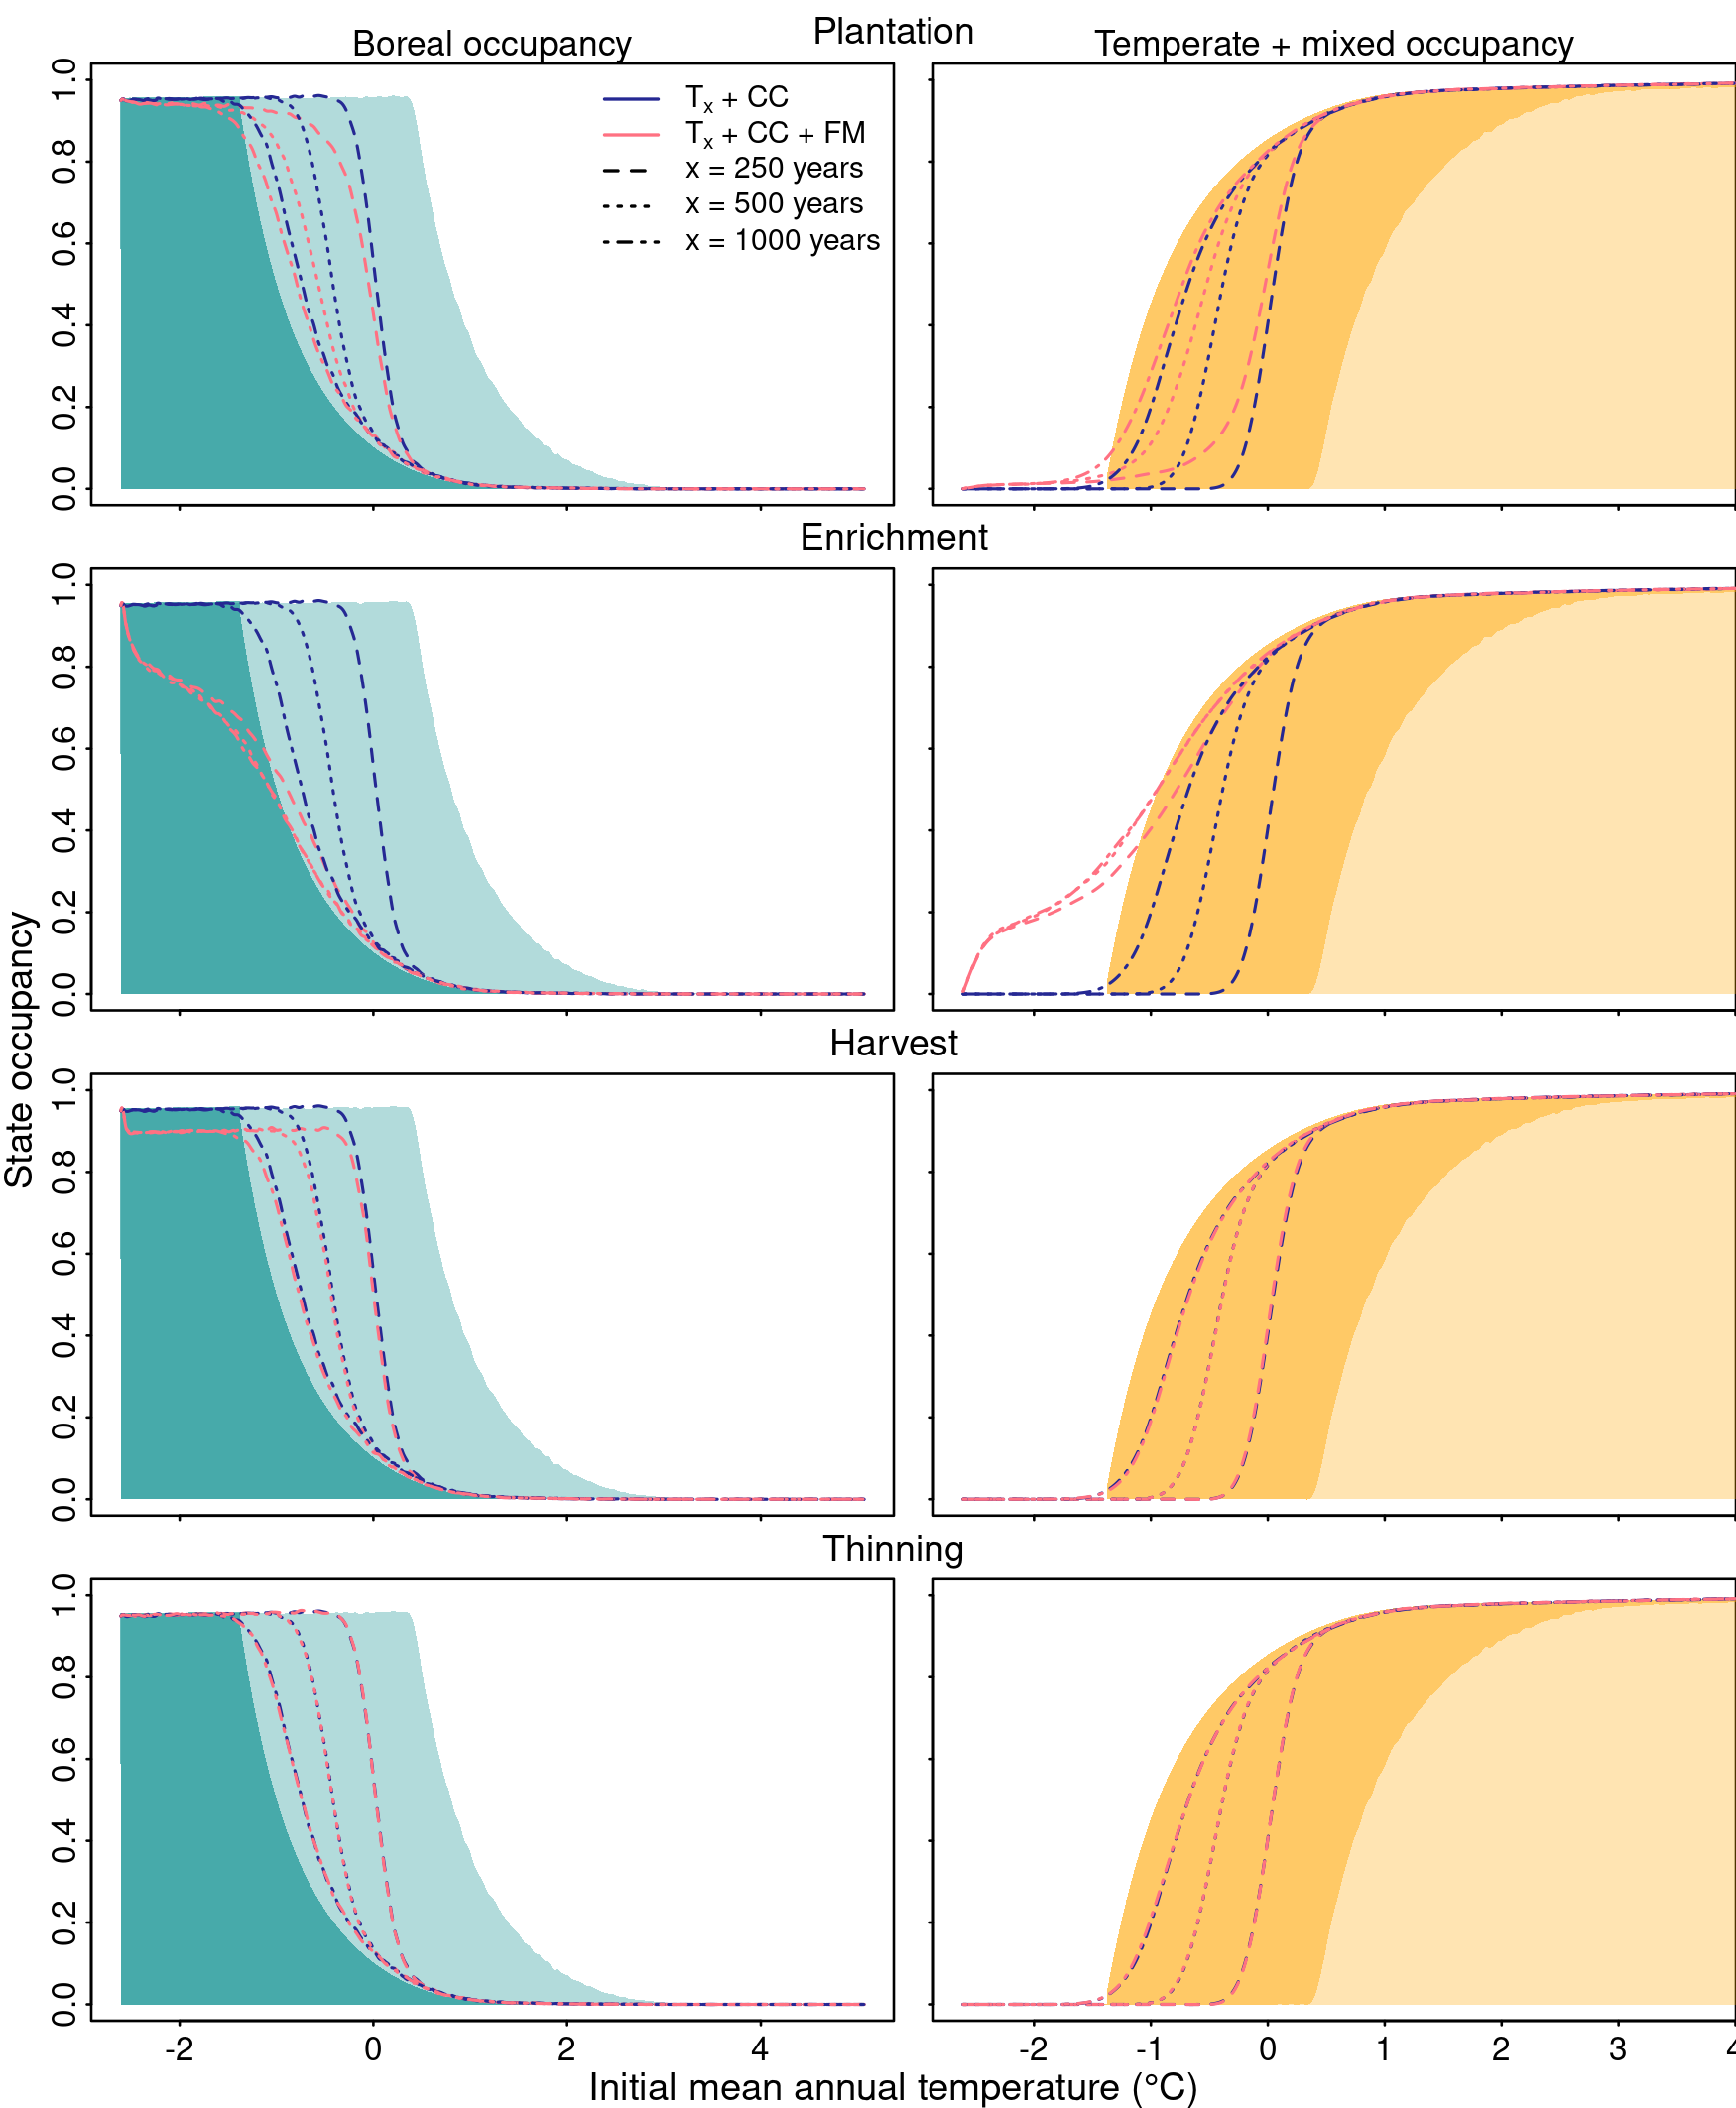
\includegraphics[width=0.79\textwidth,height=\textheight]{manuscript/img/sim-result_supp2.png}
\caption[{Boreal (left panels) and temperate plus mixed (right panels)
occupancy along the initial mean annual temperature gradient of the
boreal-temperate ecotone.}]{Boreal (left panels) and temperate plus
mixed (right panels) occupancy along the initial mean annual temperature
gradient of the boreal-temperate ecotone. Light and dark shaded areas
are a reference of the state occupancy at equilibrium before and after
warming temperature, respectively. Each line is a different simulation
to differentiate the isolated and interacting effects of climate change
(CC) and forest management (FM) for a simulation time of 250, 500, and
1000 years. Management intensity was set to 0.25\% for plantation,
thinning and enrichment planting, and 1\% for harvest. The results are
the mean of 15 replications. Confidence intervals are omitted for the
sake of simplicity.}
\label{fig:sim-result-supp4_ch1}
\end{figure}
}

\newpage

\hypertarget{fig:sim-result-supp5_ch1}{%
\begin{figure}
\centering
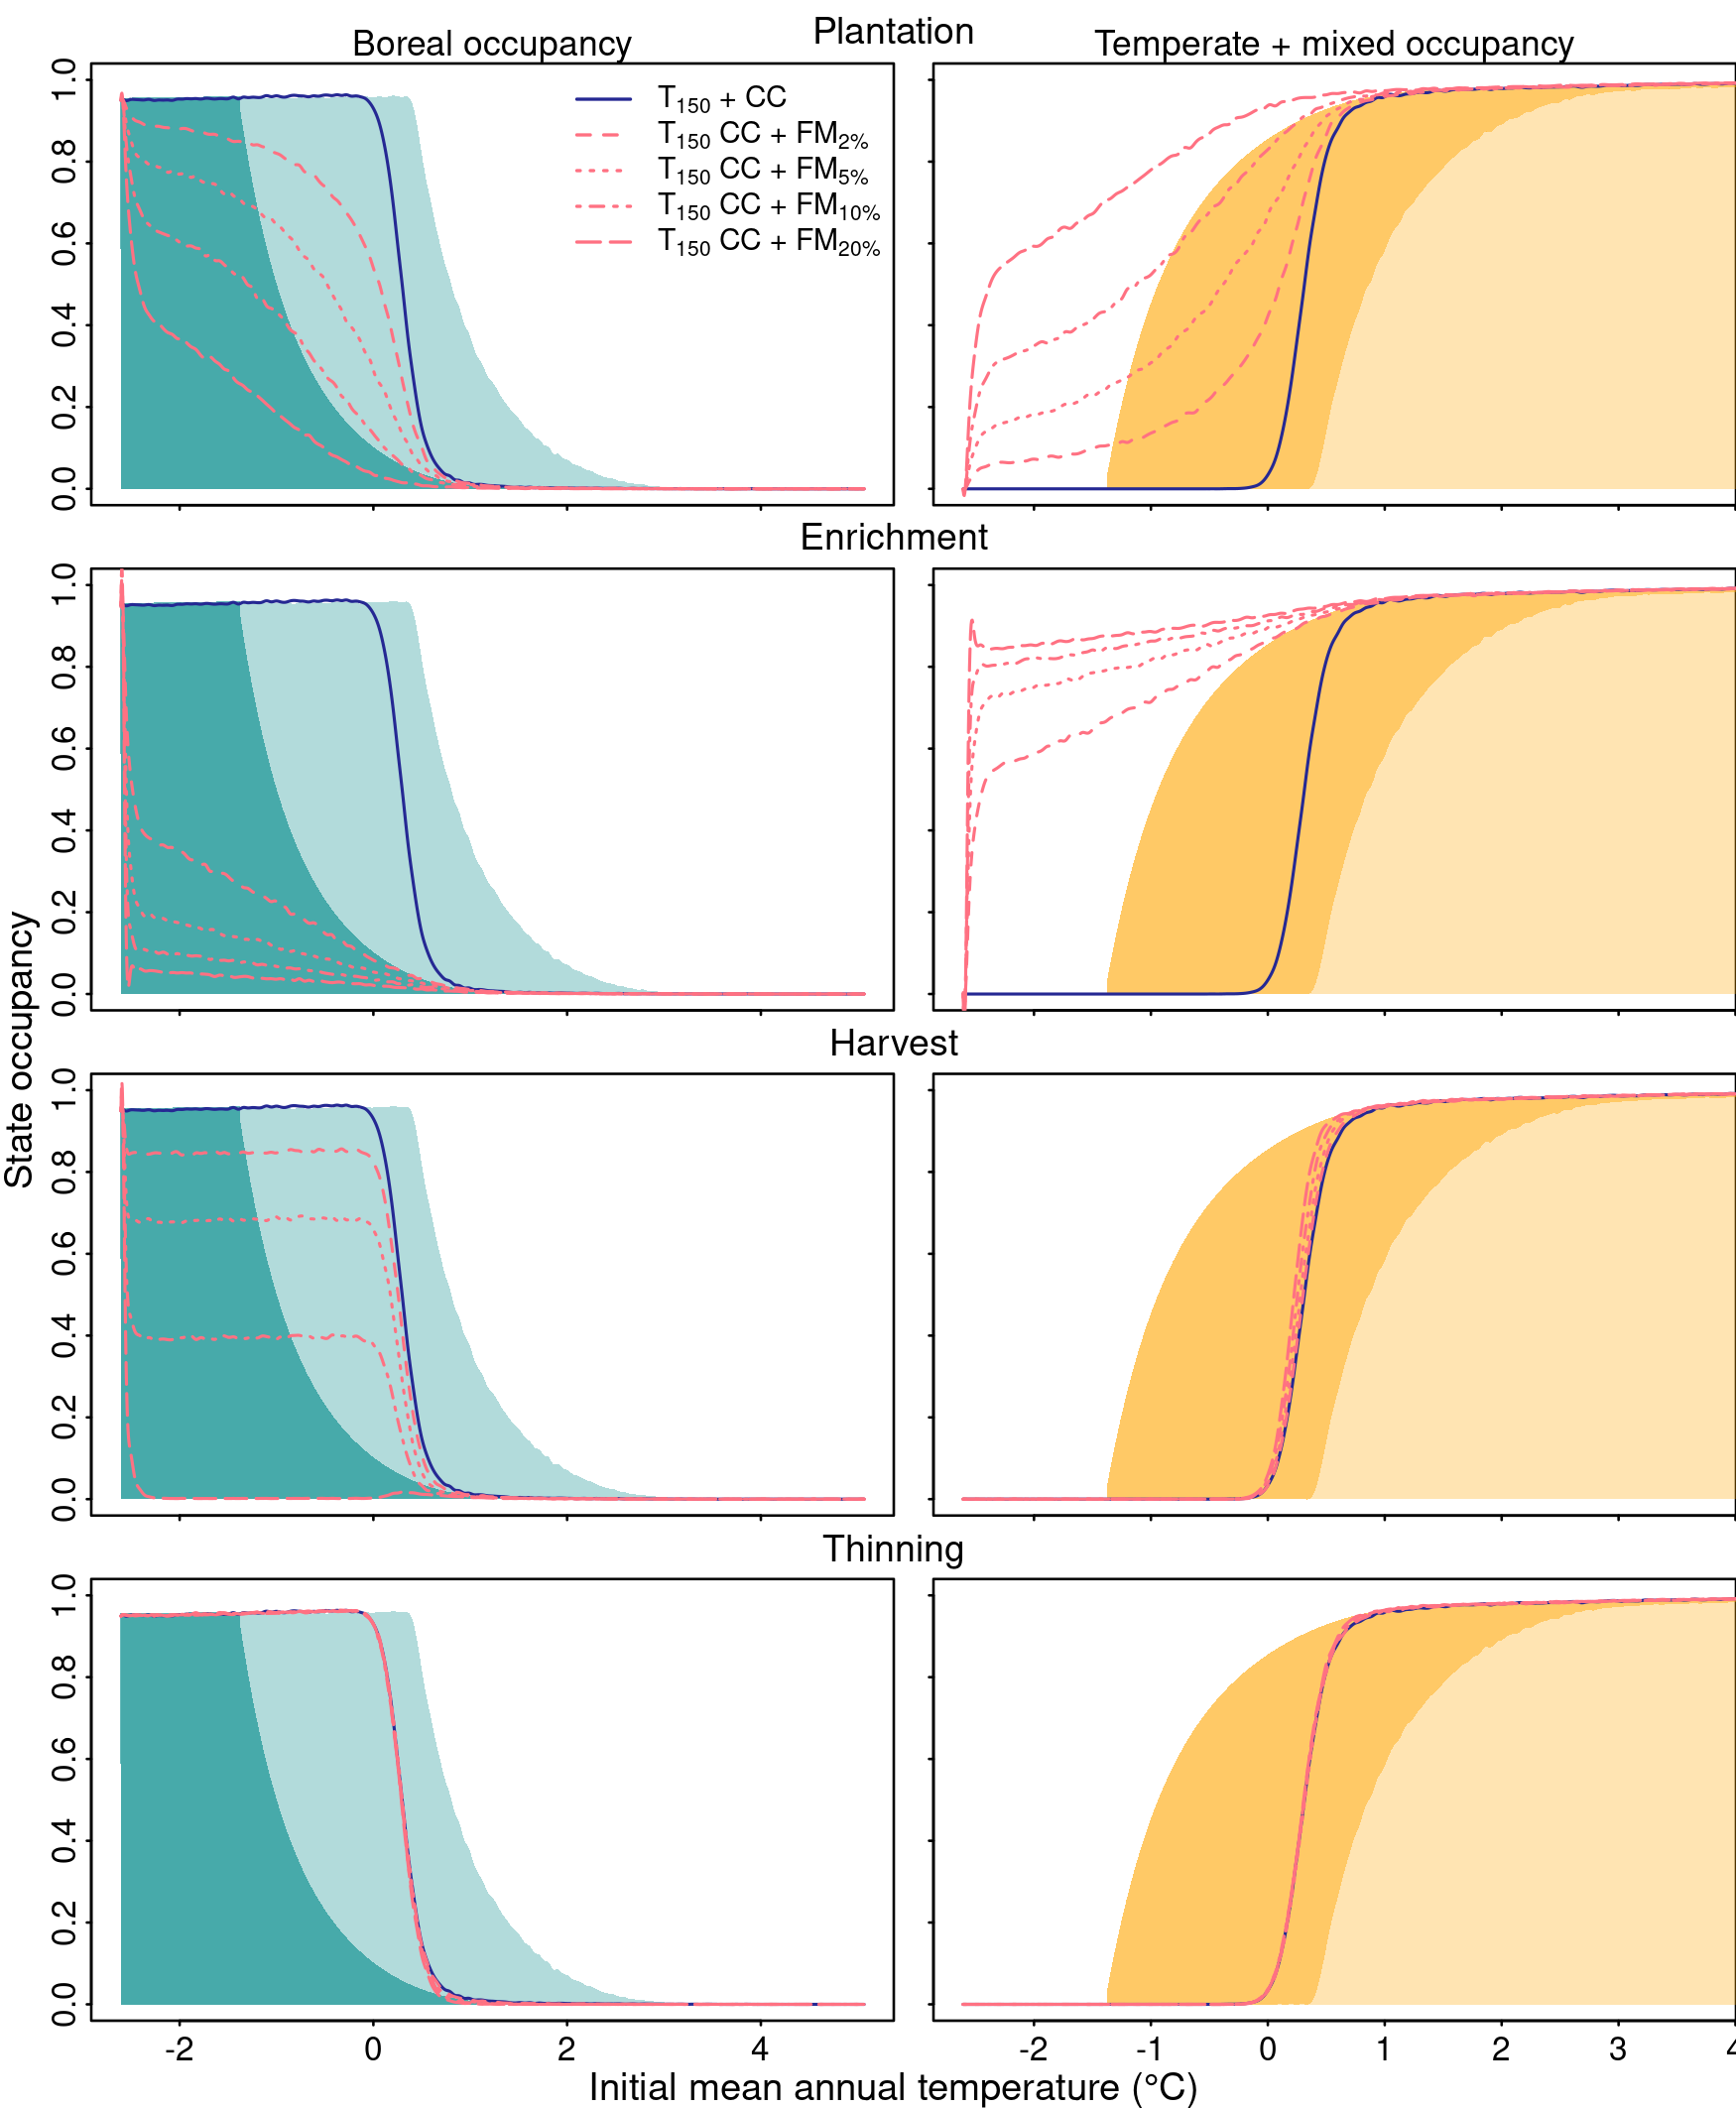
\includegraphics[width=0.79\textwidth,height=\textheight]{manuscript/img/sim-result_supp3.png}
\caption[{Boreal (left panels) and temperate plus mixed (right panels)
occupancy along the initial mean annual temperature gradient of the
boreal-temperate ecotone.}]{Boreal (left panels) and temperate plus
mixed (right panels) occupancy along the initial mean annual temperature
gradient of the boreal-temperate ecotone. Light and dark shaded areas
are a reference of the state occupancy at equilibrium before and after
warming temperature, respectively. Each line is a different simulation
to differentiate the isolated and interacting effects of climate change
(CC) and forest management (FM) with intensity of 2, 5, 10 and 20\%.
Simulation time was set to 150 years. The results are the mean of 15
replications. Confidence intervals are omitted for the sake of
simplicity.}
\label{fig:sim-result-supp5_ch1}
\end{figure}
}

\newpage

\hypertarget{fig:sim-result-supp6_ch1}{%
\begin{figure}
\centering
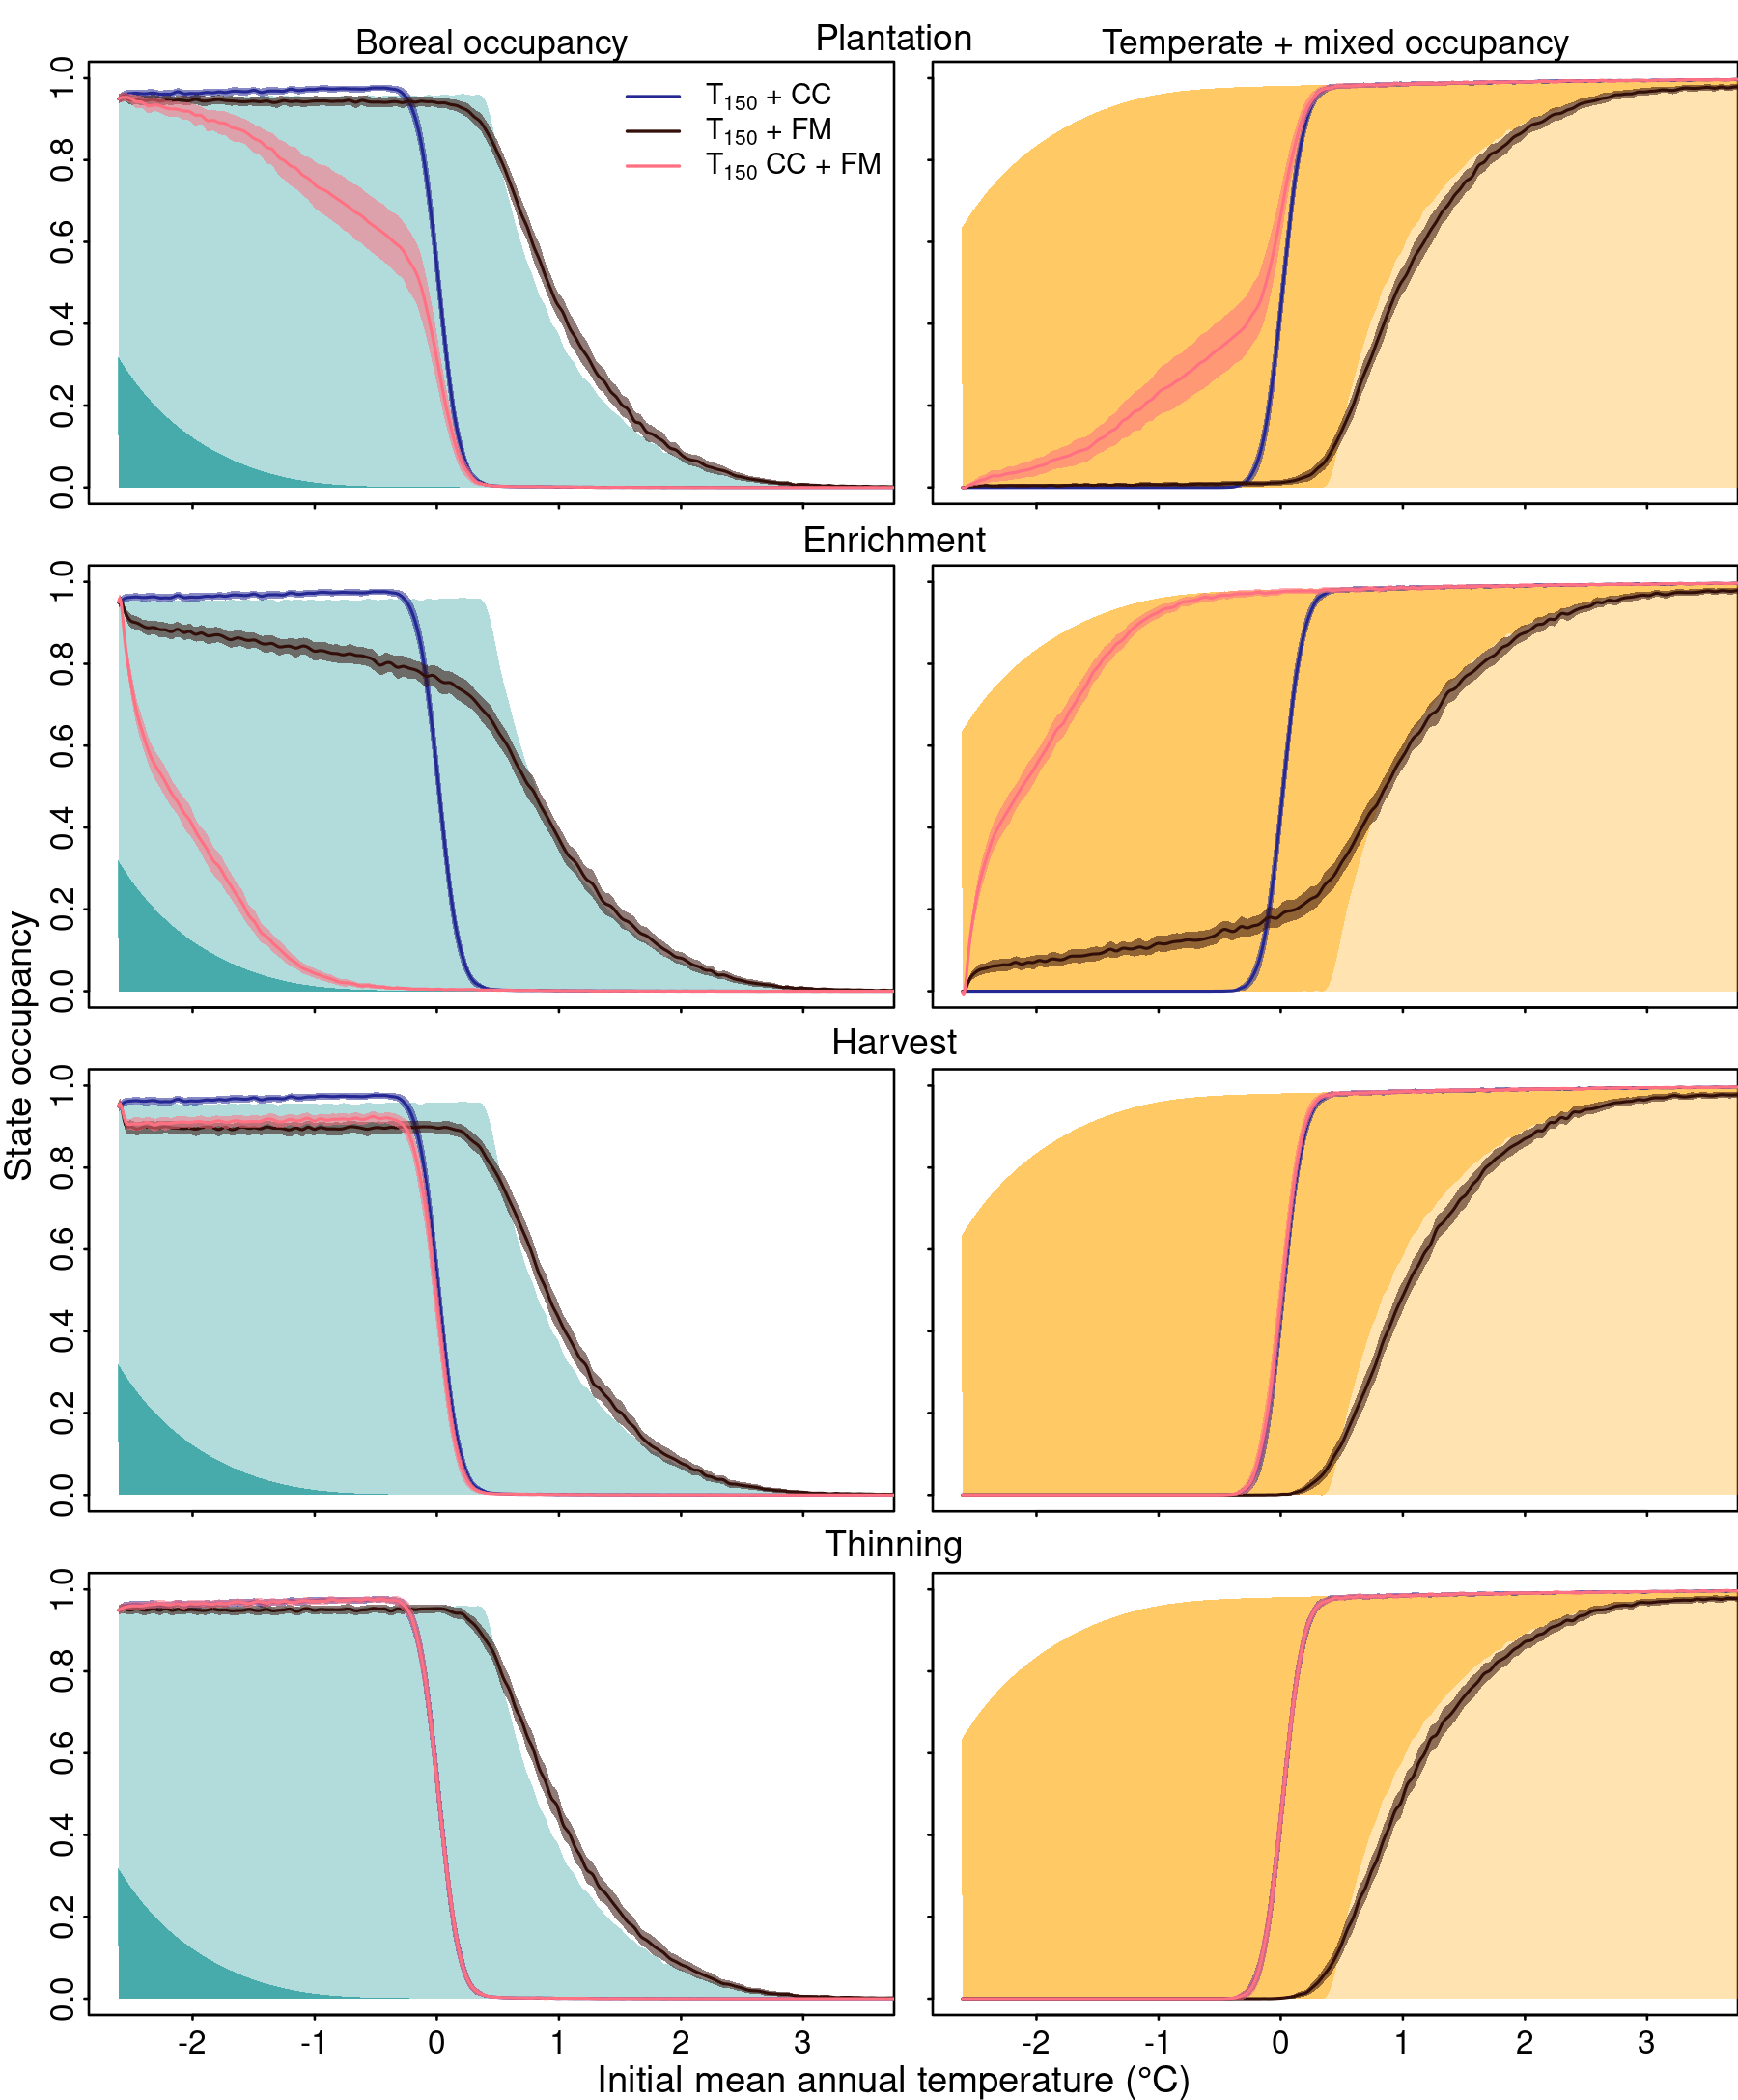
\includegraphics[width=0.75\textwidth,height=\textheight]{manuscript/img/sim-result_RCP8.5.png}
\caption[{Boreal (left panels) and temperate plus mixed (right panels)
occupancy along the initial mean annual temperature gradient of the
boreal-temperate ecotone.}]{Boreal (left panels) and temperate plus
mixed (right panels) occupancy along the initial mean annual temperature
gradient of the boreal-temperate ecotone. Light and dark shaded areas
are a reference of the state occupancy at equilibrium before and after
warming temperature, respectively. Each line is a different simulation
to differentiate the isolated and interacting effects of climate change
(CC) and forest management (FM). The results are the mean and 99\%
confidence intervals of 15 replications. Management intensity was set to
0.25\% for plantation, thinning and enrichment planting, and 1\% for
harvest, with a simulation time of 150 years. The climate change
scenario was RCP 8.5.}
\label{fig:sim-result-supp6_ch1}
\end{figure}
}

\newpage

\hypertarget{fig:sim-result-sup7_ch1}{%
\begin{figure}
\centering
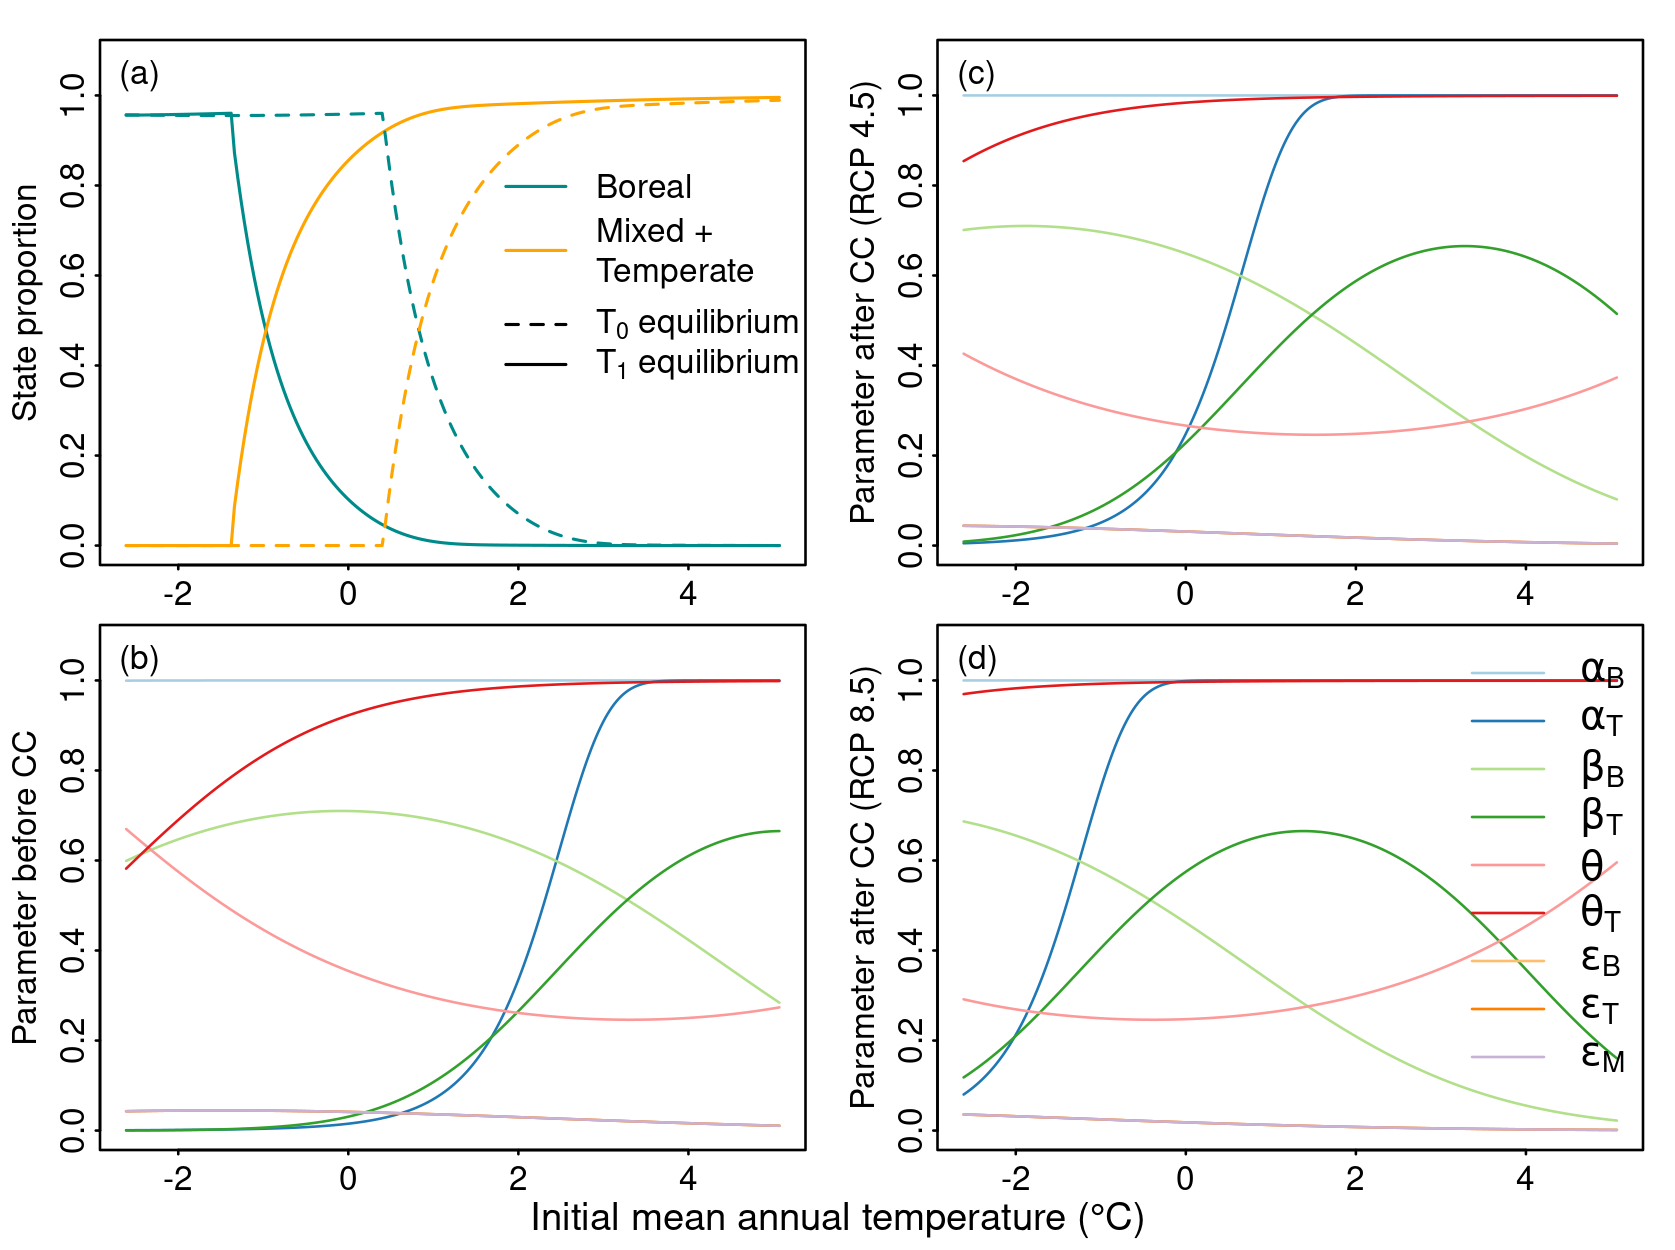
\includegraphics{manuscript/img/num-result_supp2.png}
\caption[{Parameters of the State and Transition Model varying as a
function of initial mean annual temperature from
\citet{Vissault2020}.}]{Parameters of the State and Transition Model
varying as a function of initial mean annual temperature from
\citet{Vissault2020}. Annual mean precipitation is fixed to 998.7 mm.
Parameters for (b) before and after warming temperature following (c)
RCP4.5 and (d) RCP8.5 climate change scenarios over the same latitudinal
position. Note that the \(\varepsilon_B\) and \(\varepsilon_T\) lines
are hidden behind \(\varepsilon_M\).}
\label{fig:sim-result-sup7_ch1}
\end{figure}
}

\newpage

\hypertarget{fig:sim-result-sup8_ch1}{%
\begin{figure}
\centering
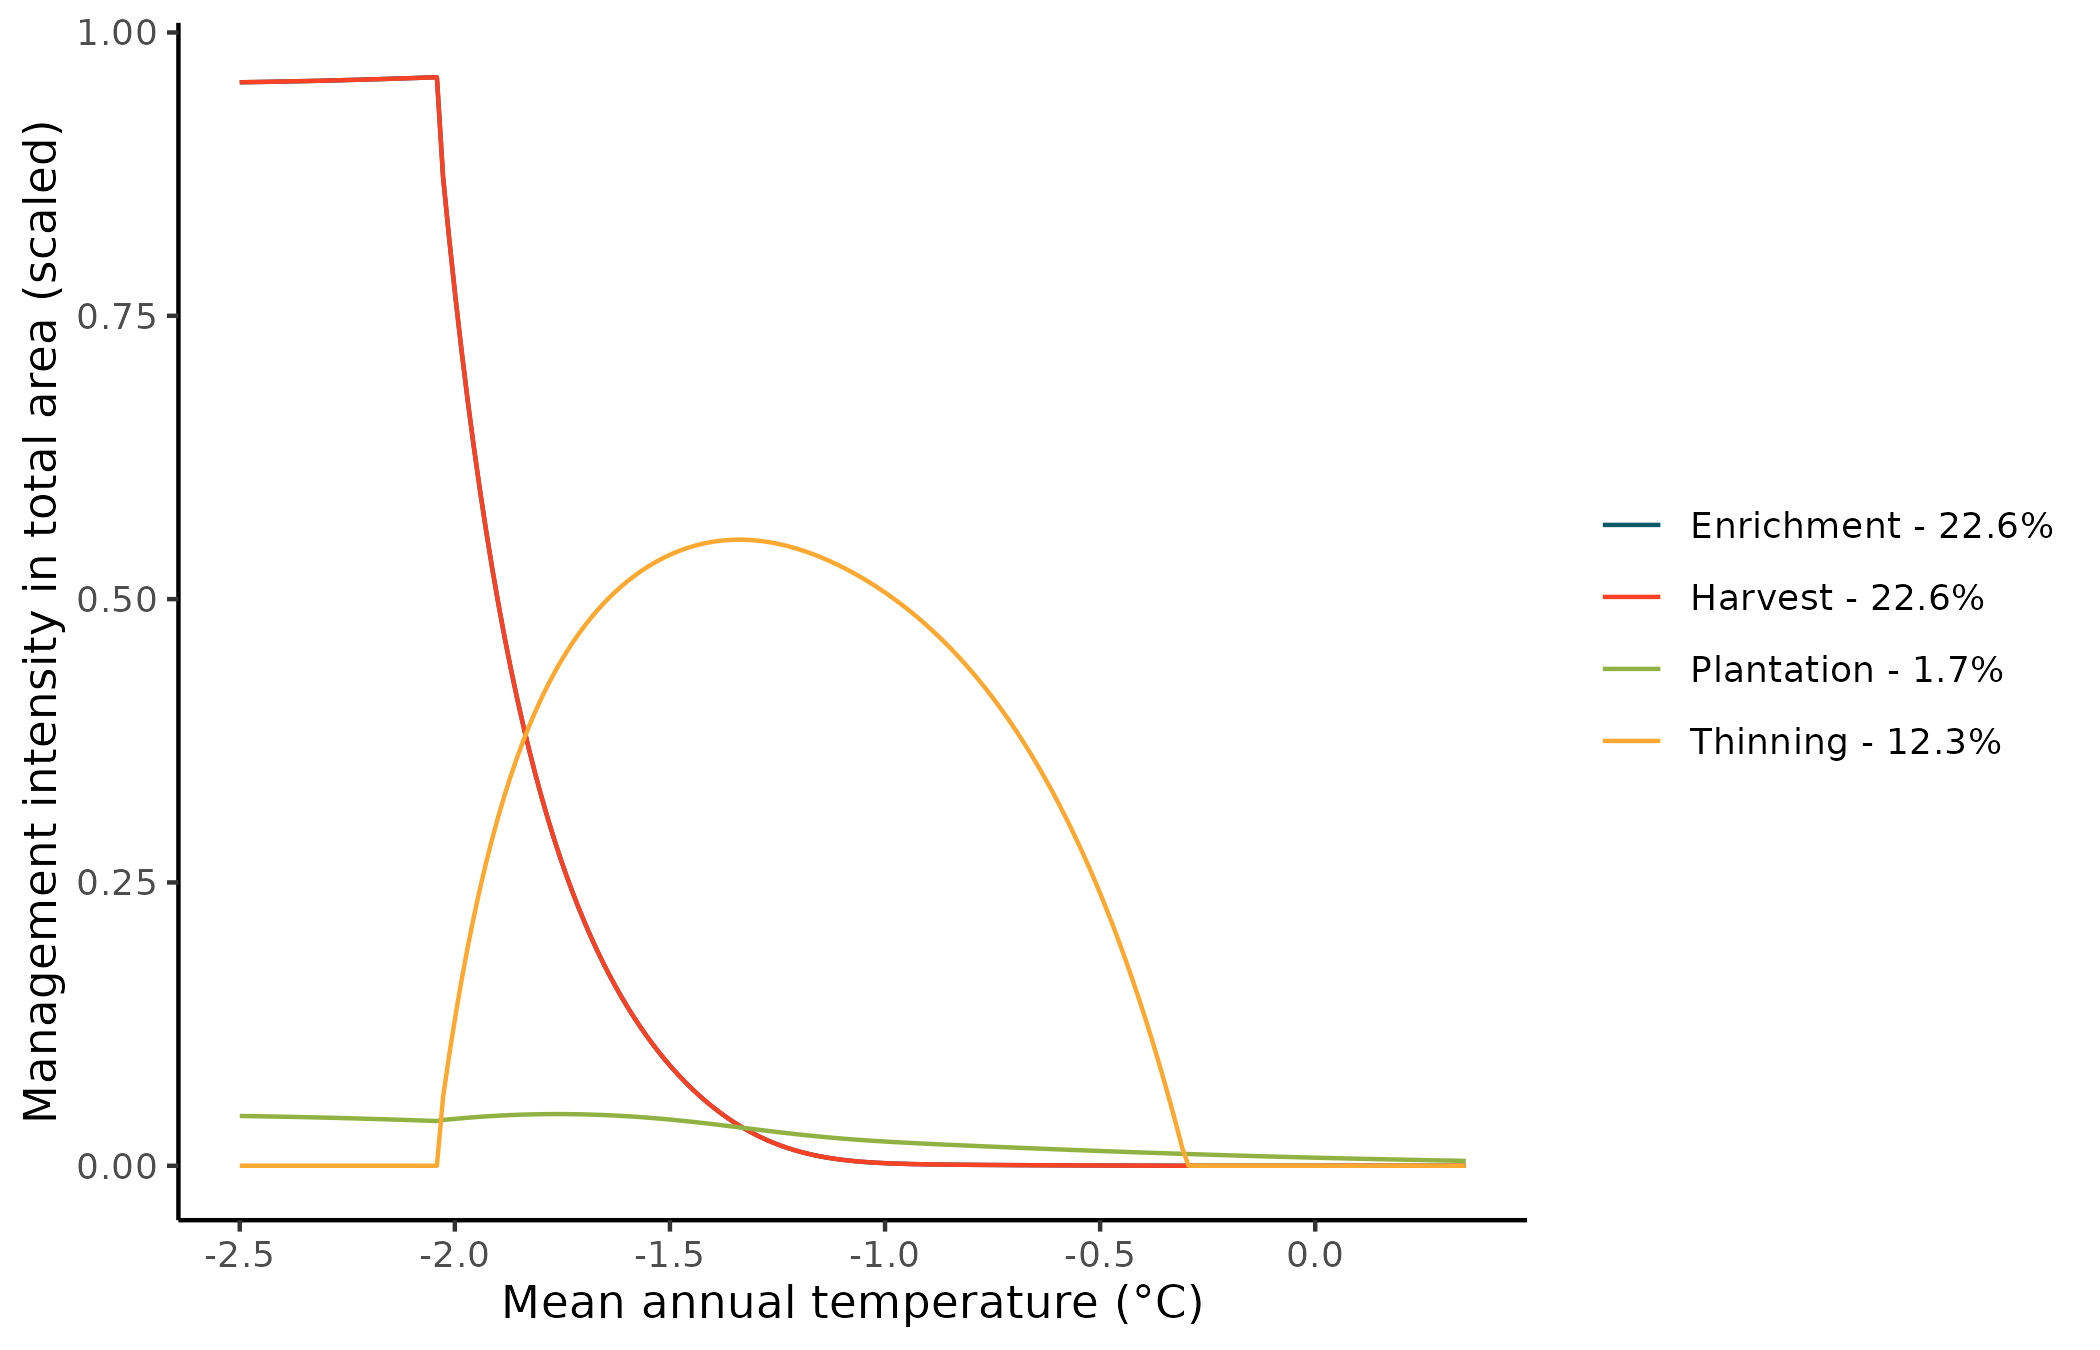
\includegraphics{manuscript/img/num-result_supp5.png}
\caption[{Distribution of management intensity adjusted by the amount of
forest state available at the equilibrium to be managed.}]{Distribution
of management intensity adjusted by the amount of forest state available
at the equilibrium to be managed. For example, at lower Mean Annual
Temperature (MAT) ranges, values close to 1 indicate that nearly 100\%
of the region is susceptible to harvesting or enrichment planting (lines
overlap). This implies that at a management intensity of 50\%,
approximately half of the landscape in that region will be affected. The
total sum of available states for management across the MAT axis is
shown in the legend.}
\label{fig:sim-result-sup8_ch1}
\end{figure}
}

\singlespacing
{\renewcommand{\bibname}{References}
\renewcommand{\bibsection}{\section{\bibname}}
\bibliography{chapter1/manuscript/references}}
\bibliographystyle{styles/myBEAS}
